%%%%%%%%%%%%%%%%%%%%%%%%%%%%%%%%%%%%%%%%%
% Simple Sectioned Essay Template
% LaTeX Template
%
% This template has been downloaded from:
% http://www.latextemplates.com
%
%
%%%%%%%%%%%%%%%%%%%%%%%%%%%%%%%%%%%%%%%%%

%----------------------------------------------------------------------------------------
%	PACKAGES AND OTHER DOCUMENT CONFIGURATIONS
%----------------------------------------------------------------------------------------
%!TEX root = 00Main.tex

%----------------------------------------------------------------------------------------
%	PACKAGES AND OTHER DOCUMENT CONFIGURATIONS
%----------------------------------------------------------------------------------------
\PassOptionsToPackage{table}{xcolor}

\documentclass[12pt]{article} % Default font size is 12pt, it can be changed here

\usepackage[margin=1.2in,footskip=1cm]{geometry} % Required to change the page size to A4
\geometry{a4paper} % Set the page size to be A4 as opposed to the default US Letter
\usepackage{textcomp}
\usepackage{lipsum}
\usepackage{graphicx} % Required for including pictures
\usepackage{amsmath}
\DeclareMathOperator*{\argmin}{arg\,minimize}
\usepackage{courier}
\usepackage{bm} %boldsymbol mathmode
% \usepackage{nccmath} %Smaller fonts for big matrices
\usepackage{float} % Allows putting an [H] in \begin{figure} to specify the exact location of the figure
\usepackage{wrapfig} % Allows in-line images such as the example fish picture
% \usepackage{pgfgantt}
\usepackage{subcaption}
\usepackage{parskip} %Read in blank lines in text (allows for paragraphs)
\usepackage[super,numbers,sort&compress]{natbib}
\renewcommand*{\thefootnote}{(\arabic{footnote})} %Change footnote styling to avoid confusion with citations
\usepackage{array}
\usepackage{tikz}
\usepackage{xcolor}
\usepackage{listings} %Typesetting code
\usepackage{fancyhdr}	%Headers and footers
\usepackage{titlesec}	%Alter titles
\usepackage{sectsty}	
\usepackage{calc}
\usepackage{abstract}
\usepackage{appendix}
\usepackage[usenames,dvipsnames]{pstricks}
\usepackage{epsfig}
\usepackage{multirow}
\usepackage{longtable}
\usepackage[nottoc,numbib]{tocbibind}
\usepackage{multicol}
\usepackage{nicefrac}
\usepackage[greek.ancient,english]{babel}
\usepackage{gensymb}
\usepackage{mcode}
\usepackage{scrextend}
\usepackage{dsfont}
\usepackage{tikz}
\usepackage{booktabs}
\usepackage{hyperref}   % Hyperlinking
\usepackage{cleveref} % Has to be loaded last

%%%%%%%%%%%%%%%%%%%%%%%%%%%%  Defining colours  %%%%%%%%%%%%%%%%%%%%%%%%%%%%

\definecolor{BioEngTeal}{rgb}{0.43529411764,0.79607843137,0.82352941176}
\definecolor{BioEngGrey}{rgb}{0.56862745098,0.5725490196,0.58431372549}
\definecolor{mygreen}{RGB}{28,172,0} % color values Red, Green, Blue
\definecolor{mylilas}{RGB}{170,55,241}
\definecolor{RubineRed}{RGB}{206,0,88}

%%%%%%%%%%%%%%%%%%%%%%%%%%%%%%%%%%%%%%%%%%%%%%%%%%%%%%%%%%%%%%%%%%%%%%%%%%%%%

%%%%%%%%%%%%%%%%%%%%%%%%%%%  New environment for typesetting big matrices  %%%%%%%%%%%%%%%%%%%%%%%%

\newenvironment{mbmatrix}{\begin{medsize}\begin{bmatrix}}%
{\end{bmatrix}\end{medsize}}%

%%%%%%%%%%%%%%%%%%%%%%%%%%%%%%%%%%%%%%%%%%%%%%%%%%%%%%%%%%%%%%%%%%%%%%%%%%%%%%%%%%%%%%%%%%%%%%%%%%%%%

%%%%%%%%%%%%%%%%  Change colours of sections, subsections, figures and tables  %%%%%%%%%%%%%%%%%

\sectionfont{\color{BioEngTeal}}  % sets colour of sections
\subsectionfont{\color{BioEngGrey}}  % sets colour of subsections
\renewcommand{\abstractnamefont}{\color{BioEngTeal}\textbf}


\renewcommand{\bibname}{References}
\renewcommand{\thefigure}{\textcolor{BioEngTeal}{\bfseries\itshape\thesection.\arabic{figure}\,}}
\renewcommand{\thesubfigure}{\textcolor{BioEngTeal}{\bfseries\alph{subfigure}}}
\renewcommand{\figurename}{\textcolor{BioEngTeal}{\bfseries\itshape Figure}}
\renewcommand{\thetable}{\textcolor{BioEngTeal}{\bfseries\itshape\thesection.\arabic{table}}}
\renewcommand{\tablename}{\textcolor{BioEngTeal}{\bfseries\itshape Table}}
\renewcommand{\theequation}{\textcolor{BioEngTeal}{\bfseries\itshape\thesection.\arabic{equation}\,}}

\addto\captionsenglish{\renewcommand{\figurename}{\textcolor{BioEngTeal}{\bfseries\itshape Figure}}}
\addto\captionsenglish{\renewcommand{\tablename}{\textcolor{BioEngTeal}{\bfseries\itshape Table}}}
%%%%%%%%%%%%%%%%%%%%%%%%%%%%%%%%%%%%%%%%%%%%%%%%%%%%%%%%%%%%%%%%%%%%%%%%%%%%%%%%%%%%%%%%%%%%%%%%%




%%%%%%%%%%%%%%%%%%%%%%%%%%%%%%% Define macro for C++ symbol  %%%%%%%%%%%%%%%%%%%%%%%%%%%%%%%%%%%%

\newcommand{\CC}{C\nolinebreak\hspace{-.05em}\raisebox{.4ex}{\bf +}\nolinebreak\hspace{-.10em}\raisebox{.4ex}{\bf +}\,\,}
\def\CC{{C\nolinebreak[4]\hspace{-.05em}\raisebox{.4ex}{\bf ++}}\,\,}

%%%%%%%%%%%%%%%%%%%%%%%%%%%%%%%%%%%%%%%%%%%%%%%%%%%%%%%%%%%%%%%%%%%%%%%%%%%%%%%%%%%%%%%%%%%%%%%%%


%%%%%%%%%%%%%%%%%%%%%%%%%%  Defining norm symbol  %%%%%%%%%%%%%%%%%%%%%%

\newcommand{\norm}[1]{\left\lVert#1\right\rVert}

%%%%%%%%%%%%%%%%%%%%%%%%%%%%%%%%%%%%%%%%%%%%%%%%%%%%%%%%%%%%%%%%%%%%%%%%


%%%%%%%%%%%%%%%%%%%%%%%%%%%%%%%%%  Defining footer  %%%%%%%%%%%%%%%%%%%%%%%%%%%%%%%%%%

\pagestyle{fancy}
\fancyhf{}
\renewcommand{\footrulewidth}{0.5pt}
\renewcommand{\headrulewidth}{0pt}

\fancyfoot[R]{\color{BioEngTeal}\textbf{\thepage}}
\fancyfoot[L]{\raisebox{-.75\height}{\includegraphics[scale=1]{Pictures/bioengineering_logo_left.eps}}}

%%%%%%%%%%%%%%%%%%%%%%%%%%%%%%%%%%%%%%%%%%%%%%%%%%%%%%%%%%%%%%%%%%%%%%%%%%%%%%%%%%%%%%





%%%%%%%%%%%%%%%%%%%%%%%  Change font to Helvetica %%%%%%%%%%%%%%%%%%%%%%%%%%%

% % Include the helvet package
% \usepackage{helvet}

% % Set the default font to be sans-serif
% \renewcommand*{\familydefault}{\sfdefault}
% \makeatletter
% \newcommand{\thickhline}{%
%     \noalign {\ifnum 0=`}\fi \hrule height 2pt
%     \futurelet \reserved@a \@xhline
% }
% \newcolumntype{"}{@{\hskip\tabcolsep\vrule width 1pt\hskip\tabcolsep}}
% \makeatother
%%%%%%%%%%%%%%%%%%%%%%%%%%%%%%%%%%%%%%%%%%%%%%%%%%%%%%%%%%%%%%%%%%%%%%%%%%%%%%%%%%%%%

%%%%%%%%%%%%%%%%%%%%%%%  Fonts  %%%%%%%%%%%%%%%%%%%%%%%%%%%
\usepackage[scale=.75]{sourcecodepro} % monospace font
\usepackage{courier}
\renewcommand{\ttfamily}{pcr}
\usepackage{gfsbaskerville}
\usepackage[osf]{Baskervaldx} % tosf in text, tlf in math
\usepackage[T1]{fontenc}
% \usepackage[baskervaldx,cmintegrals,bigdelims,vvarbb]{newtxmath} % math italic letters from Baskervaldx
% \usepackage[cal=boondoxo]{mathalfa} % mathcal from STIX, unslanted a bit
% \usepackage{ebgaramond-maths}
%%%%%%%%%%%%%%%%%%%%%%%%%%%%%%%%%%%%%%%%%%%%%%%%%%%%%%%%%%%%%%%%%%%%%%%%%%%%%%%%%%%%%

\linespread{1.2} % Line spacinggit gitg

\setlength\parindent{0pt} % Uncomment to remove all indentation from paragraphs

\graphicspath{{Pictures/}} % Specifies the directory where pictures are stored

%%%%%%%%%%%%%%%%%%%%%%%%%%%%%%%%%%%%%%%%%%%%%%%%%%%%%%%%%%%%%%%%%%%%%%%%%%%%%%%%%%%%%%



%%%%%%%%%%%%%%%%%%%%%%%%%%%%%  Typesetting code  %%%%%%%%%%%%%%%%%%%%%%%%%%%%%%%%%%%%%
\definecolor{listinggray}{gray}{0.9}
\definecolor{lbcolor}{rgb}{0.9,0.9,0.9}
\definecolor{Darkgreen}{rgb}{0.13,0.545,0.13}

\usepackage[numbered,framed]{matlab-prettifier}

\usepackage{filecontents}

\let\ph\mlplaceholder % shorter macro
\lstMakeShortInline"

\lstset{
  style              = Matlab-editor,
  basicstyle         = \mlttfamily,
  escapechar         = ",
  mlshowsectionrules = true,
}


% Command for placeholder
\newcommand\placeholder[1]%
{%
    \bgroup
        \normalfont\upshape\color{RubineRed}%
        < {\itshape #1\/} >%
    \egroup
}


% Command for error
\newcommand\error[1]%
{%
    \bgroup
        \color{red}%
        #1\/
    \egroup
}



\lstset
{%
    escapechar=`,
}
%%%%%%%%%%%%%%%%%%%%%%%%%%%%%%%%%%%%%%%%%%%%%%%%%%%%%%%%%%%%%%%%%%%%%%%%%%%%%%%%%%%%%%%%
\begin{document}


\hrule

\begin{figure}[t]
	\begin{subfigure}[b]{0.40\linewidth} 					
    \includegraphics[height=0.8cm]{logo.jpg}     
  \end{subfigure}
    \hfill
	\begin{subfigure}[B]{0.40\linewidth} 						
    \includegraphics[height=0.8cm]{Pictures/bioengineering_logo_right.eps}
  \end{subfigure}
    \hfill
\end{figure}

\vspace{1cm}


\begin{center}
{\large \textbf{Mini-project 2019: Image processing}} % Title of your document
\end{center}
The purpose of this mini-project is to consolidate all that you have learned about MATLAB so far. After completing this project you should feel confident in tackling computational problems using MATLAB.

\section{Marking}
This project will \textbf{not} be counted towards your overall grade, but your performance will be taken into consideration when you are choosing projects in the third and fourth year. You may discuss your understanding of the problems and solutions with your peers but you must not share your solution code. Your marks will be based entirely on the runtime performance of your code. Although there are no marks for comments, you are advised to include them so that you can quickly recapture your thought processes at some distant future time, for example at a job interview.
The marks out of 100 are displayed in the header for each exercise. 

You are not required to submit anything for this mini-project. You will be assessed on your performance during the final session on either \textbf{20 June 2019} or \textbf{21 June 2019}. When you have finished, please ask for a teaching assistant to examine your code.
\section{Overview}
In this project you will be writing code to process medical images. Imagine you are part of a team that develops medical analysis software and you have been tasked to code some of the functions which should fit into a larger programme.  You are required to write two functions:

\begin{enumerate}
	\item one function to rotate an image and
	\item another function to detect edges in an image,
\end{enumerate}

\subsection{Rotation [70]}
Write a function named \mcode{rotate_image}, this function should take a matrix representing a grayscale image as input and should output a rotated version of the image as another matrix. In addition it should take another input which specifies the angle to rotate the image at, given in radians. Thus, the function should have the following signature:

\begin{minipage}{\textwidth}
\begin{lstlisting}
function [output_image] = rotate_image(input_image, theta)
\end{lstlisting}
\end{minipage}

Image rotation can be achieved by performing what is called a reverse mapping operation. You take the rotated image and for each pixel of the rotated image, you determine where in the original image the pixel came from. Mathematically, this can be expressed as:

\begin{equation}
	\begin{bmatrix}
		x_{output} \\
		y_{output}	
	\end{bmatrix}	
	= 
	\begin{bmatrix}
		cos(\theta) & sin(\theta) \\
		-sin(\theta) & cos(\theta)
	\end{bmatrix}^{-1}
	*
	\Bigg(
	\begin{bmatrix}
		x_{input} \\
		y_{input}
	\end{bmatrix}
	-
	\begin{bmatrix}
		x_{centre} \\
		y_{centre}
	\end{bmatrix}
	\Bigg)
	+
	\begin{bmatrix}
		x_{centre} \\
		y_{centre}
	\end{bmatrix}
	,
\end{equation}
where ($x_{input}$, $y_{input}$) are the coordinates for a pixel in the input (un-rotated) image and ($x_{output}$, $y_{output}$) are the coordinates of the output (rotated) image.
The extra terms involving the coordinates for the centre of the image ($x_{centre}$, $y_{centre}$) are included because we want the rotation to occur around the centre of the image and not the origin. The angle $\theta$ is the angle of the rotation given in radians.

The following shows the expected behaviour of the function given an image called \mcode{test_image}:

\begin{minipage}{\textwidth}
\begin{lstlisting}
clear all

% Load the image
load mri % Demo image within MATLAB
test_image = D(:,:,:,1);

% Rotate the image by pi/4 radians using the function
rotated_image = rotate_image(test_image, pi/4);

% Display rotated image and original image side-by-side
figure(1) % Create figure

subplot(1,2,1) 
imagesc(test_image)
title('Original image')
axis square

subplot(1,2,2)
imagesc(rotated_image)
title('Rotated image')
axis square

colormap gray % Change the colourmap to gray
\end{lstlisting}
\end{minipage}

\begin{figure}[H]
\centering
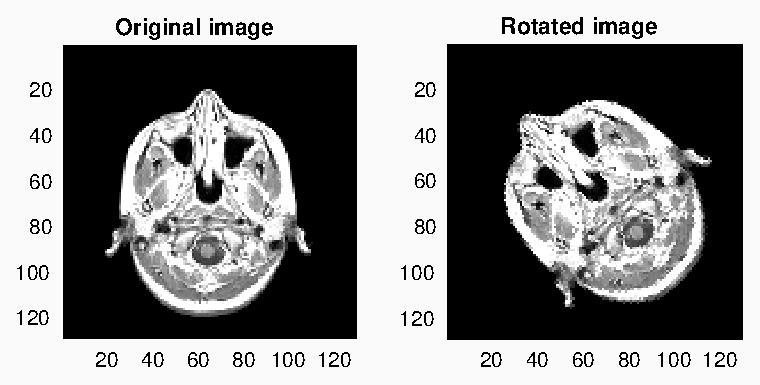
\includegraphics[width = .8\textwidth]{Pictures/rotate_example.eps}

\end{figure}

\subsection{Edge detection [30]}
Write a function named \mcode{detect_edges}, which takes a grayscale image as input and outputs the edges of that image as another image. The function signature should look like the following:

\begin{minipage}{\textwidth}
\begin{lstlisting}
function [output_image] = detect_edges(input_image)
\end{lstlisting}
\end{minipage}

A simple way to perform edge detection is by using a two pass approach: 
\begin{enumerate}
	\item one pass through the image to look for horizontal edges and
	\item one pass through the image to look for vertical edges.
\end{enumerate}

The result of these two passes is then averaged to yield the final image. In other words:

$$ Out_{horizontal}(x, y) = \left|In(x, y) - In(x+1, y)\right|$$ 
$$ Out_{vertical}(x, y) = \left|In(x, y) - In(x, y+1)\right|$$
$$ Out(x,y) = \frac{Out_{horizontal}(x, y)+Out_{vertical}(x, y)}{2}$$
where $Out$ and $In$ denote the output and input image respectively. $\left| x \right|$ denotes the absolute value function.
The expected behaviour:
\begin{figure}[H]
\centering
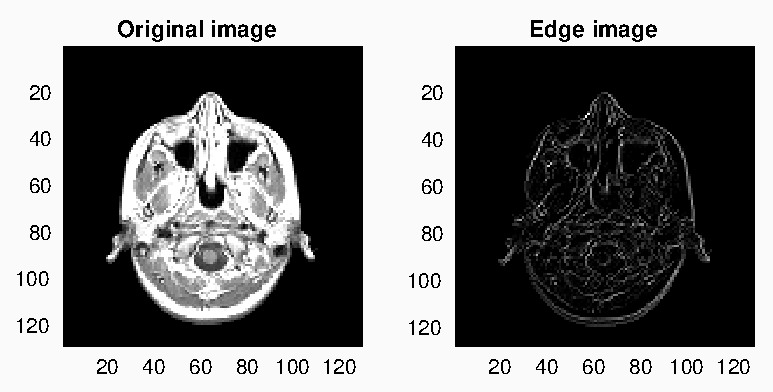
\includegraphics[width = .8\textwidth]{Pictures/edge_detect_example.eps}

\end{figure}

% \subsection{Blurring}
% Lastly, write a function which takes an input image and outputs a blurred version of it. Call this function \mcode{blur_image}, with the following input signature:

% \begin{minipage}{\textwidth}
% \begin{lstlisting}
% function [output_image] = blur_image(input_image)
% \end{lstlisting}
% \end{minipage}

% Blurring can be achieved by averaging a pixel with its neighbouring pixels. We can write this as:

% $$ Out(x,y) = \frac{\sum^2_{i=0}\sum^2_{j=0} In(x+i, y+j)}{9} $$
% where $Out$ and $In$ denote the output and input image respectively. This should result in the following blur effect:

% \begin{figure}[H]
% \centering
% 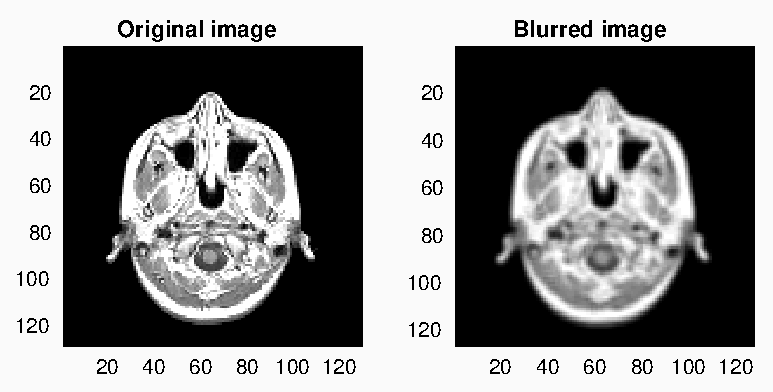
\includegraphics[width = .8\textwidth]{Pictures/blur_example.eps}

% \end{figure}

\subsection{(Optional) Vectorisation}
Try rewriting both \mcode{detect_edges} and \mcode{blur_image} to use vectorisation instead of loops. Investigate the difference in execution time between your original code and the vectorised code. Call these functions \mcode{detect_edges_vectorised} and \mcode{blur_image_vectorised}.

\end{document}

